\documentclass[conference]{IEEEtran}
\IEEEoverridecommandlockouts
% The preceding line is only needed to identify funding in the first footnote. If that is unneeded, please comment it out.
\usepackage{cite}
\usepackage{amsmath,amssymb,amsfonts}
\usepackage{algorithmic}
\usepackage{graphicx}
\usepackage{textcomp}
\usepackage{xcolor}
\graphicspath{ {./} }
\def\BibTeX{{\rm B\kern-.05em{\sc i\kern-.025em b}\kern-.08em
    T\kern-.1667em\lower.7ex\hbox{E}\kern-.125emX}}
\begin{document}

\title{Toxic issues in Github\\}

\maketitle

\begin{abstract}
Abstract 
\end{abstract}

\begin{IEEEkeywords}
Keywords 
\end{IEEEkeywords}

\section{Introduction}
Introduction
\section{Related Works}
Related works 

\section{Data and Methods}
We designed a classification scheme to dientify potentially toxic issues on Github. We use our method a novel method that leverages differences between Software Engineering and English vocabularies to improve accuracy. We show that our scheme outperforms other methods, and we use this scheme in later sections to find trends in toxic comments. 

\subsection{Data}
Our source of data is the June 2019 version of GHTORRENT \cite{b2} , a database of Github issues, comments and pull requests. We had over 80M issues available to us. Each issue had metadata about its origin including creator and creation date, and the text from each of the issue's comments. 


To predict toxic issues, we created a training dataset by labeling issues and their corresponding comments. We searched through issues that were marked as "too heated," selected a random sample of 179 issues, and labeled them with 73 of the issues being toxic, and 106 labeled as non-toxic. In order to add more non-toxic issues, we took 225 random issues on github, and labeled them (all were non-toxic). Finally, we used our Active Learning procedure on 1653 random issues to label 51 more issues (20 were toxic). In the end, this resulted in our training data set having a total of 455 issues, with 93 issues being toxic, and 362 issues being non-toxic. 

We performed some pre-processing the comment text. We removed any snippets of code, and removed urls and emojis (but kept track of the number of urls and emojis per comment). 


For each comment, we kept track of heuristics and also used external libraries to evaluate comments. A full of table of features we considered is below. 

\begin{table}[]
	\begin{tabular}{ll}
		\textbf{Feature} & \textbf{Description}                                                                                        \\
		Num Emojis       & Number of Emojis                                                                                            \\
		Num Urls         & Number of URLs                                                                                              \\
		Length           & Length in Characters                                                                                        \\
		Stanford Polite  & Using CITATION we give a 0-1 score of politeness, where 0 is the least polite, and 1 is the most polite     \\
		Perspective      & Using CITATION, we give a 0-1 score of how toxic comments are, where 0 is the least toxic and 1 is the most \\
		Subjectivity     & Using TextBlob sentiment, get a 0-1 score of subjectivity, where 1 is the most subjective                   \\
		Polarity         & Using TextBlob sentiment, get a -1-1 score of polarity, where 1 and -1 are the most subjective              \\
		NLTK Score       & Using VADER sentiment analyzer (CITATION), we find the compound sentiment score                             \\
		TF IDF           & Use TF IDF word frequencies                                                                                 \\
		Anger            & Number of words from Anger Lexicon (CITATION)                                                               \\
		Negative         & Number of words from Negative Lexicon (CITATION)                                                           
	\end{tabular}
\end{table}

\subsection{Model} 

We use an SVM classifier to classify comments as toxic or non-toxic. We then classify issues by defining toxic issues to be those with at least one toxic comment. Our SVM classifier has two hyperparameters, C and $\gamma$. We vary these hyperparameters to find the best classifier. We choose an SVM classifier because it's been commonly used for text classification (CITATION). 

In addition to the features mentioned earlier, we use three other techniques to improve the classifier's predictions. 

\textbf{Context} - Comments don't occur in a vacuum (CITATION). As a result, we try and get context from the comments immoderately preceding and following it in the discussion. We get the features for those comments, and use those in addition to the features about the current comment. If there is no surrounding comments, then the context is set to 0. 

\textbf{Anger Direction} - Many toxic classifiers pick up on phrases that indicate self directed anger (such as "I'm so stupid"). These typically do not interfere with a disccussion or make it toxic, and so they typically become false positives. We use a classifier from CITATION, that classifies the direction of anger as either self, other person or object. We use this classifier to label any comment that has self directed anger as non toxic. 

\textbf{Software Engineering Words} - There are vocabulary differences between Software Engineering and regular English. Sometimes, these issues interfere with a classifier's ability to predict a comment as toxic (such as the difference in the meaning of the word "bug"). We combat this by first finding "Software Engineering specific words", or words that are significantly more common in Software Engineering than regular English. We see whether removing each of these words from comments predicted as toxic significantly lowers the predicted toxicity, and if so, we label the comment as non-toxic. 

To determine whether a word is "Software Engineering specific", we create a corpus of Software Engineering text from randomly sampling 10K random github issues. To determine specificity, we use a Chi Squared Distribution with effect size at $phi=0.3$. To determine whether the predicition is significantly lower, we check whether the difference in perspective score between with and without the word is $<\alpha$, where $\alpha$ is a hyperparameter. 

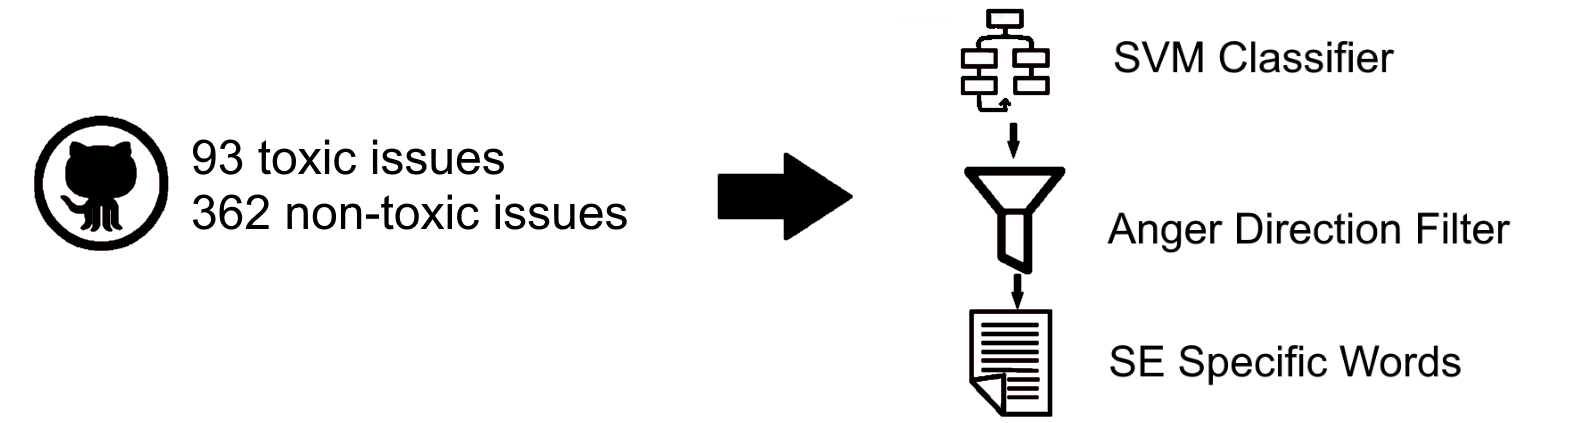
\includegraphics[width=6cm]{pipeline.png}


\subsection{Validation} 
To find the best parameters and features and validate our model, we perform 10-fold cross validation. Within each fold, we perform 10-fold cross validation on the train dataset, splitting the train dataset into a train and validation dataset (CITATION). We iteratively add features (depending on whether the model performs better) (CITATION), and we grid search hyperparameters (C=[.01,.1,1,10,100], $\gamma$=[1,2,4,8], $\alpha$=[.05,.1,.2]) and we also search over the presence/non-presence of each of the three methods from the previous subsection. We select the best hyperparameters from the train-validation split, and use that for the train-test split. To find the best set of hyperparameters overall, we pick the most common value for each hyperparameter from the train-test split. 

To quantify model performance, we use F-Scores (CITATION) at $\beta$=0.5. We use $\beta$=0.5, because we want a high precision value so that the model can accurately select toxic comments when run over large datasets. Other papers have also used $\beta$=0.5 (CITATION). 

\subsection{Validation Results} 

Validation Results



\section{Results and Discussion}
Results and Discussion

\section{Threats to Validity}
Threats to Validity

\section{Conclusion}
Conclusion

\section{References}


\begin{thebibliography}{00}
\bibitem{b1} Cohen, Jacob. Statistical power analysis for the behavioral sciences. Routledge, 2013.
\bibitem{b2} Georgios Gousios: The GHTorrent dataset and tool suite. MSR 2013: 233-236
\bibitem{b3} Gachechiladze, Daviti, et al. "Anger and its direction in collaborative software development." 2017 IEEE/ACM 39th International Conference on Software Engineering: New Ideas and Emerging Technologies Results Track (ICSE-NIER). IEEE, 2017.
\bibitem{b4} Scott, Mike, and Christopher Tribble. Textual patterns: Key words and corpus analysis in language education. Vol. 22. John Benjamins Publishing, 2006.
\bibitem{b5} Bonett, Douglas G. "Transforming odds ratios into correlations for meta-analytic research." (2007): 254.
\bibitem{b6} Görnitz, Nico, et al. "Toward supervised anomaly detection." Journal of Artificial Intelligence Research 46 (2013): 235-262.



\end{thebibliography}


\end{document}
